\documentclass[a4paper,11pt]{article}
\usepackage{graphicx,url}
\usepackage[T1]{fontenc}
\usepackage[utf8]{inputenc}
\usepackage[brazil]{babel}
\usepackage{a4wide}
\graphicspath{{./imagens/}}
\title{\vspace{-4cm}Relatório 01 - Laboratório de Arquitetura de Computadores}
\author{Luiz Junio Veloso Dos Santos - Matricula: 624037}

\begin{document} 

\maketitle

\begin{enumerate}
    \item \textbf{Circuitos no Logisim:}
        \begin{figure}[ht]
            \caption{1/2 somador}
            \centering
            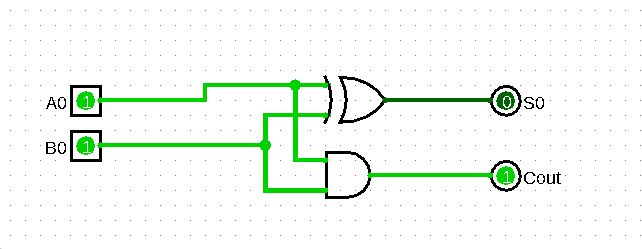
\includegraphics[width=10cm]{logisim-halfadder}
        \end{figure}                                                      
        \begin{figure}[ht]
            \vspace{-1cm}
            \caption{somador completo de 1 bit}
            \centering
            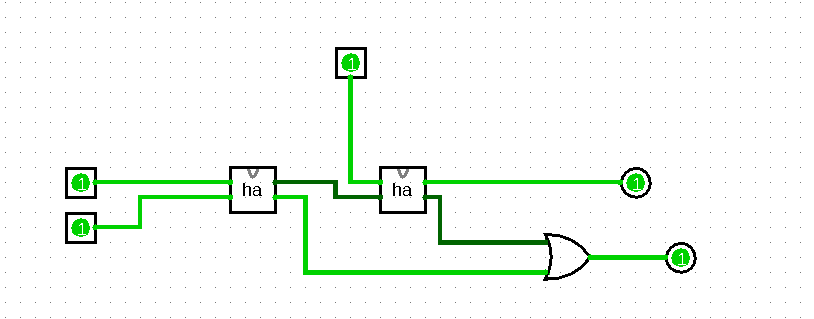
\includegraphics[width=10cm]{logisim-fulladder}
        \end{figure}                                                     
        \begin{figure}[ht]
            \vspace{-1cm}
            \caption{somador completo de 4 bits}
            \centering
            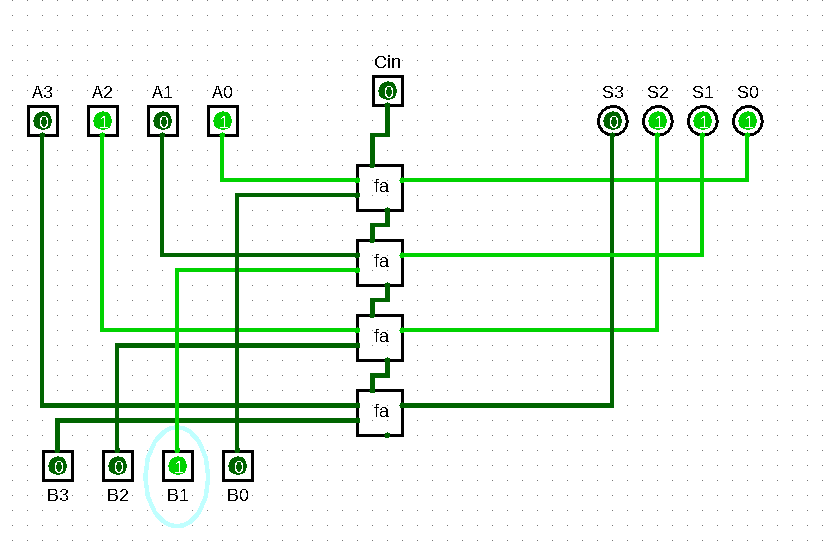
\includegraphics[width=10cm]{logisim-fulladder4}
        \end{figure}
        \newpage
    \item \textbf{Circuitos no Simulador 97:}
        \begin{figure}[ht]
            \vspace{-0.2cm}
            \caption{1/2 somador}
            \centering
            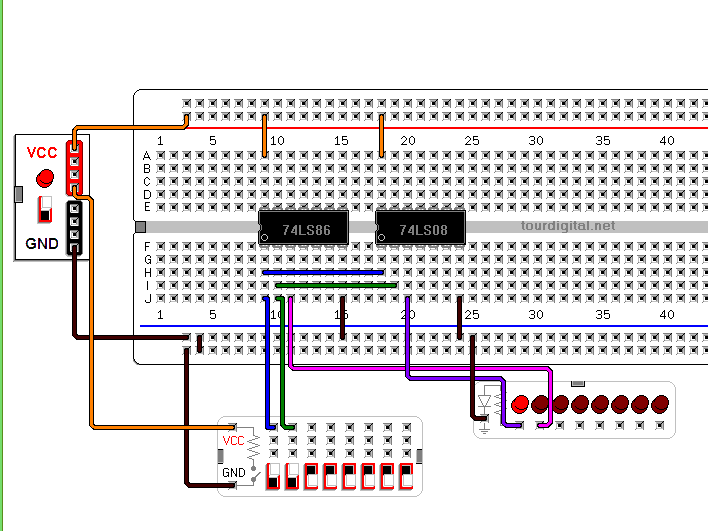
\includegraphics[width=11cm]{simulador97-meioSomador}
        \end{figure}  
        \begin{figure}[ht]
            \vspace{-1cm}
            \caption{somador completo de 1 bit}
            \centering
            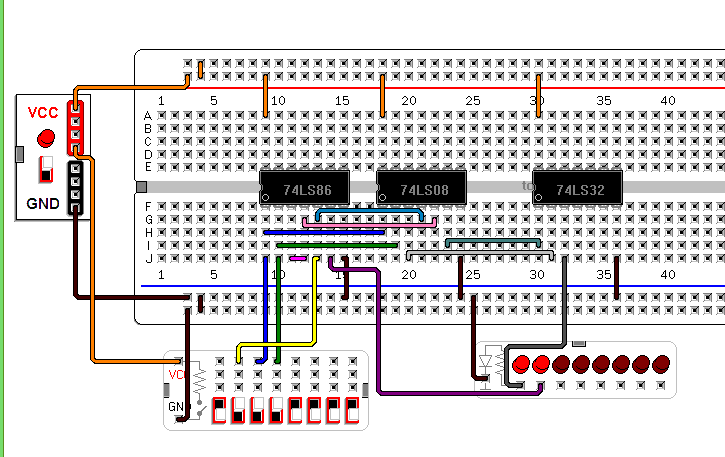
\includegraphics[width=11cm]{simulador97-somadorCompleto}
        \end{figure}
        \newpage
    \item \textbf{Perguntas:}
        \begin{enumerate}
            \item{Pergunta 1: O que acontece se um dos terminais de entrada de uma porta lógica não
                    estiver conectado em 0 ou 1 (eletricamente ele deverá estar flutuando, ou seja não
                    conectado a nenhum nível lógico)?} 
                \newline 
                \textbf{R:} Acontece desse terminal solto de comportar como nível logico 1, mas podendo
                sofrer interferências externas.
                \bigskip

            \item{Pergunta 2: Qual o problema de tempo associado a esse tipo de somador (pense no carry), considere o atraso médio de cada porta lógica de 10ns.}
                \newline
                \textbf{R:} O problema de tempo associado a esse tipo de somador, está na dependência do Carry
                In com a soma anterior, sendo necessário a espera dele até o fim do circuito para que a soma
                esteja concluída.
                \bigskip

            \item{Pergunta 3: Qual o tempo necessário para a computação de uma soma e do vai um em um somador
                    de 4 bits?}
                \newline
                \textbf{R:} O tempo necessário para a computação de uma soma em um somador completo de 4 bits
                é de 80ns e do "vai um" é 90ns no total.
                \newline
                No primeiro somador completo de 1bit a soma leva 10ns
                da XOR/AND + 10ns do outro XOR/AND + 10ns da OR responsável pela saída do "Vai um" que é necessário
                para a continuação da soma de 4 bits.
                \newline
                No segundo somador não é considerado o tempo do primeiro
                conjunto de XOR/AND, pois ocorre simultaneamente com os demais, logo o segundo somador vai
                demorar 10ns do segundo conjunto de XOR/AND (que é dependente do carry in) + 10ns da OR
                necessária para o carry out dar continuação a soma.
                \newline
                O terceiro somador completo irá demorar o mesmo que o segundo.
                \newline
                Já o quarto somador, ele irá demorar 10ns do segundo conjunto de XOR/AND para completar a
                soma. Mas o carry out ainda demora mais 10ns da OR.
                \newline
                Por isso a soma em um somador completo de
                4 bits irá demorar 80ns, mas o "vai um" irá  demorar os 80ns + 10ns do Último carry out, que
                para a soma de 4bits não é necessária no resultado.
                \bigskip

            \item{Pergunta 4: O que seria necessário para um somador de 32 bits?}
                \newline
                \textbf{R:} Para construir um somador de 32 bits seria necessário 32 somadores de 1 bit, ou 8 somadores de 4 bits, ou 4 somadores de 8 bits.
                \bigskip
            \item{Pergunta 5: Considerando esses tempos acima, calcule a frequência de operação de um somador
                    de 32 bits.}
                \newline 
                Um somador completo de 32 bits irá demorar 30ns + 31*20ns, considerando o ultimo carry out.
                Logo:
                $$ t = 30ns + 31 * 20ns = 650ns $$
                $$ f = 1 / t $$
                $$ f = 1 / 6,5 * 10^{-7} $$
                $$ f = 1.538 Mhz $$
                \bigskip
            \item{Pergunta 6: Você consegue propor alguma forma de tornar essa soma mais veloz?}
                \newline
                \textbf{R:} Separava a soma do carry, para remover ou diminuir essa espera.
                \bigskip
        \end{enumerate}
\end{enumerate}

\end{document}
